\section{Results}

\subsection{Gaze Tracking}
For our gaze tracking component, we investigated a few different approaches to gaze tracking as documented in the survey of gaze tracking performed by 
\begin{figure}[H]
    \centering
    \begin{minipage}{.5\textwidth}
      \centering
      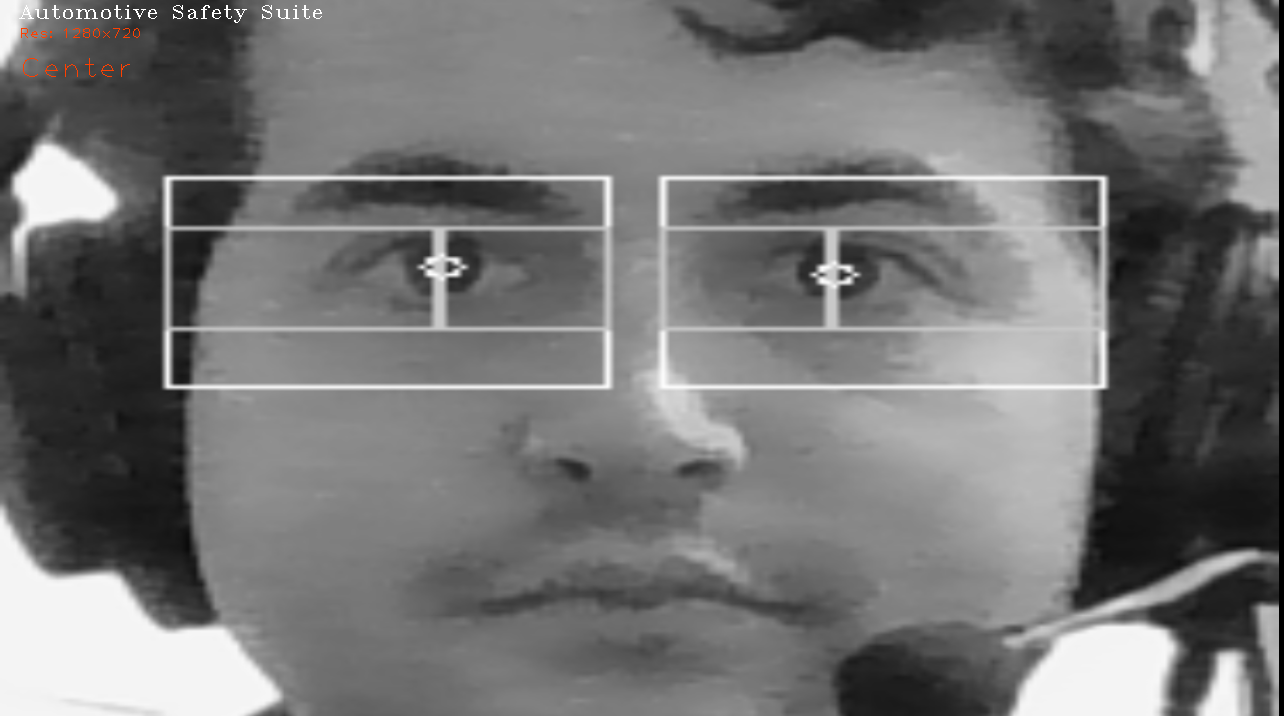
\includegraphics[width=\linewidth]{figures/EyeTrackingStraight.png}
      \captionof{figure}{Gaze tracking, straight. In the top lefthand corner of the window is the current eye tracking state}
      \label{fig:test1}
    \end{minipage}%
    \begin{minipage}{.5\textwidth}
      \centering
      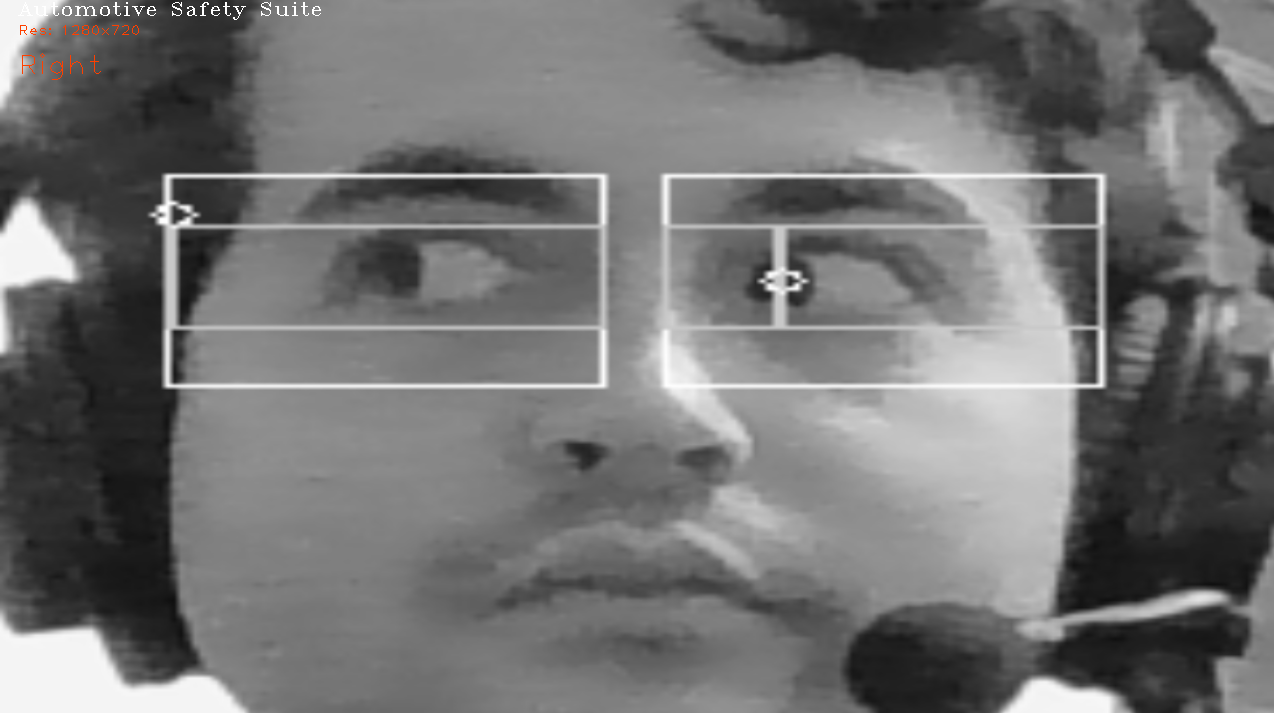
\includegraphics[width=\linewidth]{figures/EyeTrackingRight.png}
      \captionof{figure}{Gaze tracking, right. In this example the left bounding box mistook the dark region of hair as a pupil}
      \label{fig:test2}
    \end{minipage}
\end{figure}

\subsection{Pedestrian Tracking}
The original testing results when testing with a laptop camera were a little lackluster. For the most part, the use of the HOG descriptor using this wecam resulted in inaccurate readings of human objects within the frame. Mostly it would detect human-like objects in the negative space between objects. An example of this would be when someone was standing reasonably far away from the camera and the HOG descriptor would identify human-shaped objects in the armpits of the subject standing in front of the camera or in the surrounding spaces. Another example is when the subject was standing in front of the camera with their hand turned sideways. This issue arose because the quality of the camera used produced a significant amount of noise in each frame resulting in changes in gradients.\\



\begin{figure}[H]
    \begin{subfigure}[b]{.49\textwidth}
    \centering
    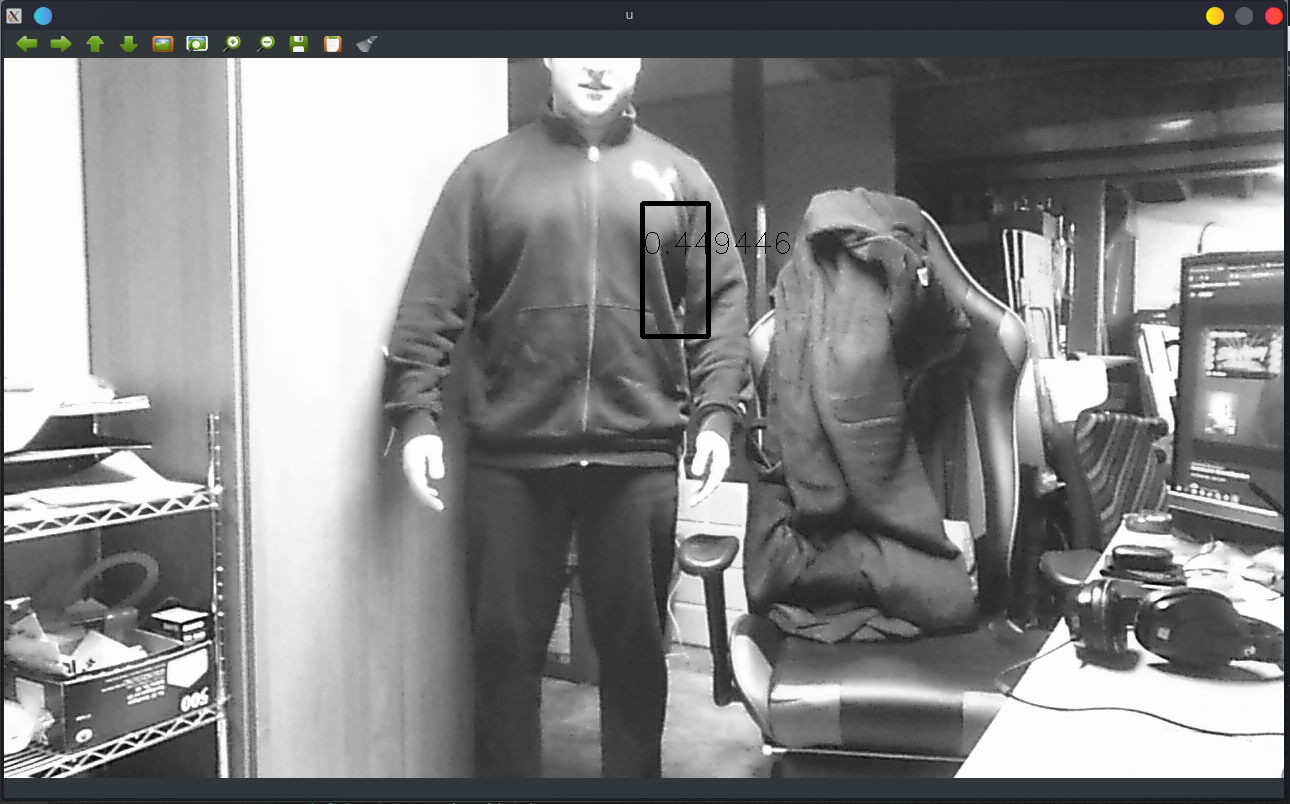
\includegraphics[width=\textwidth]{figures/PT_webcam_armpit.png}
    \caption{Detected Armpit Error}
    \end{subfigure}\hfill
    \begin{subfigure}[b]{.49\textwidth}
    \centering
    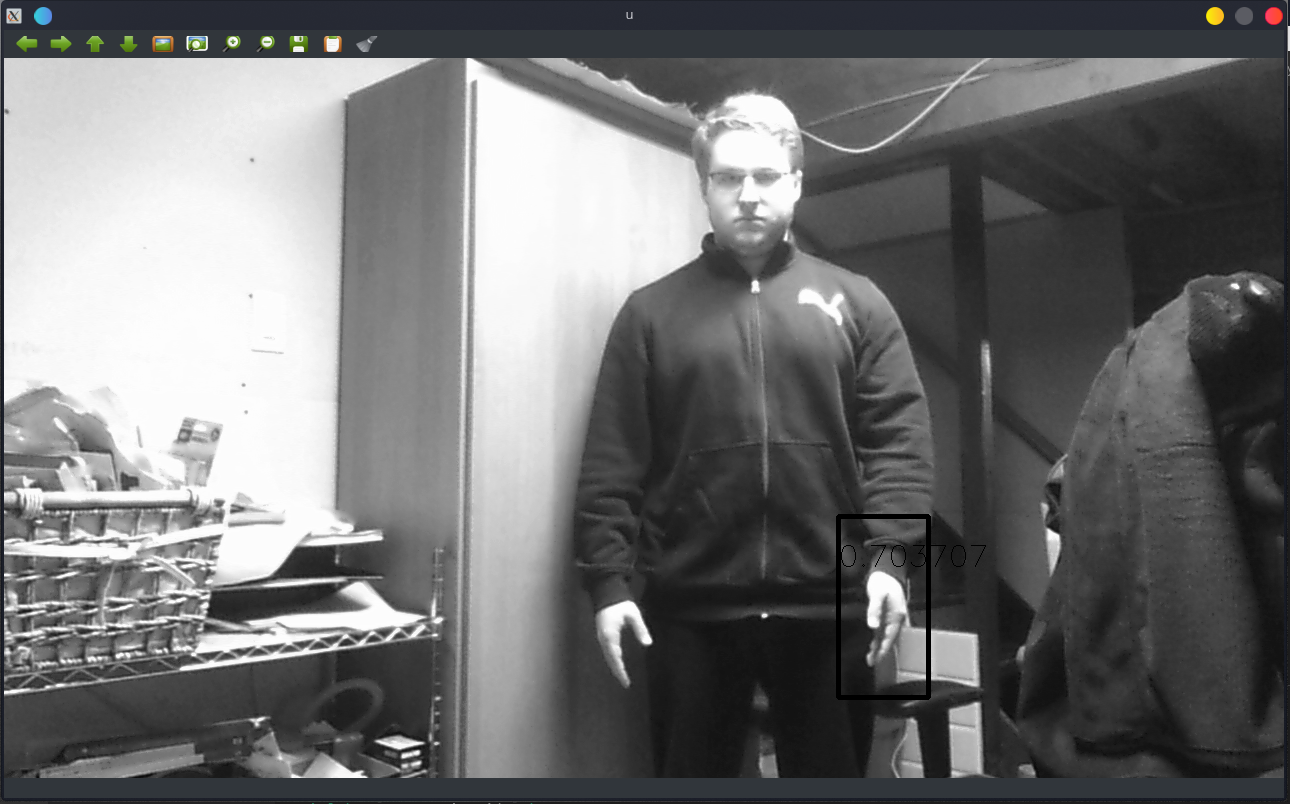
\includegraphics[width=\textwidth]{figures/PT_webcam_hand.png}
    \caption{Detected Hand Error}
    \end{subfigure}%
    \caption{Errors produced using a noisy webcam}
\end{figure}
% \begin{figure}[H]
%     \centering
%     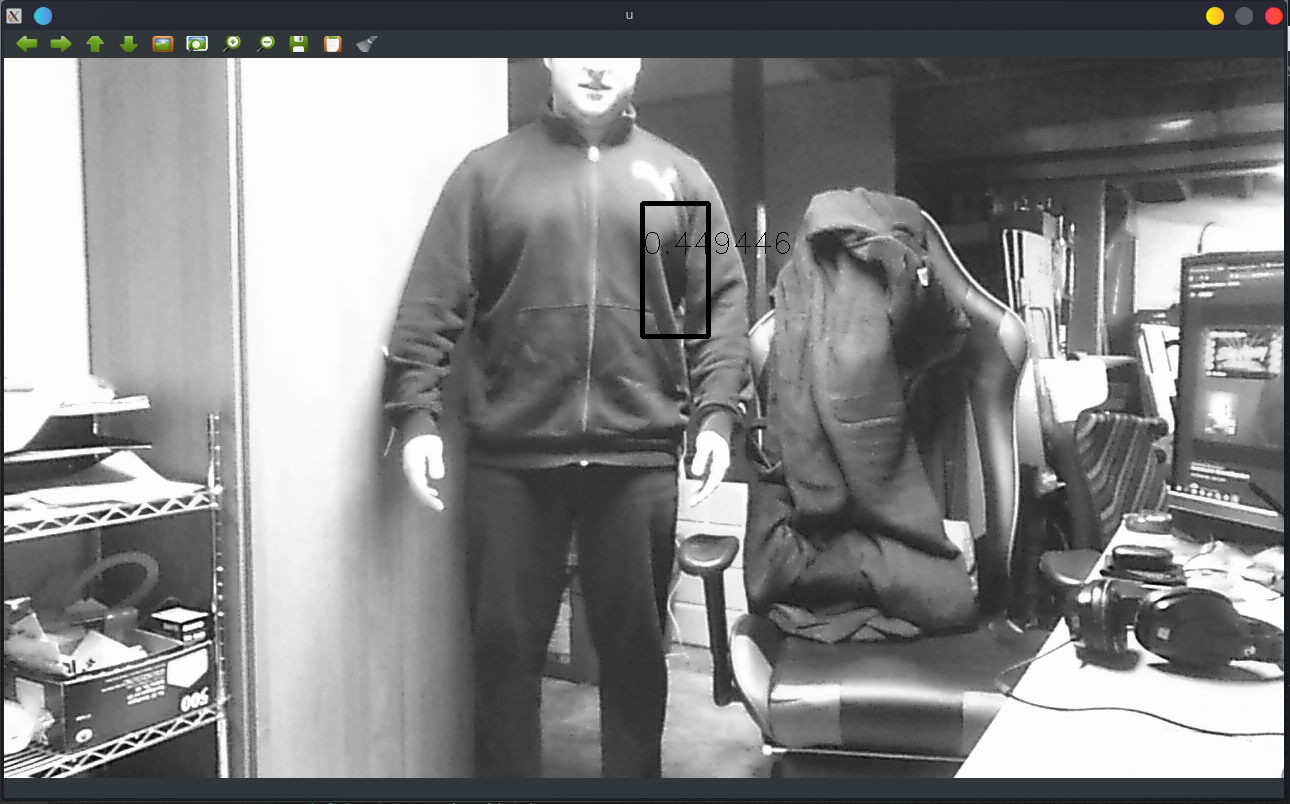
\includegraphics[width=\textwidth]{figures/PT_webcam_armpit.png}
%     \caption{Armpit Detection Error}

%     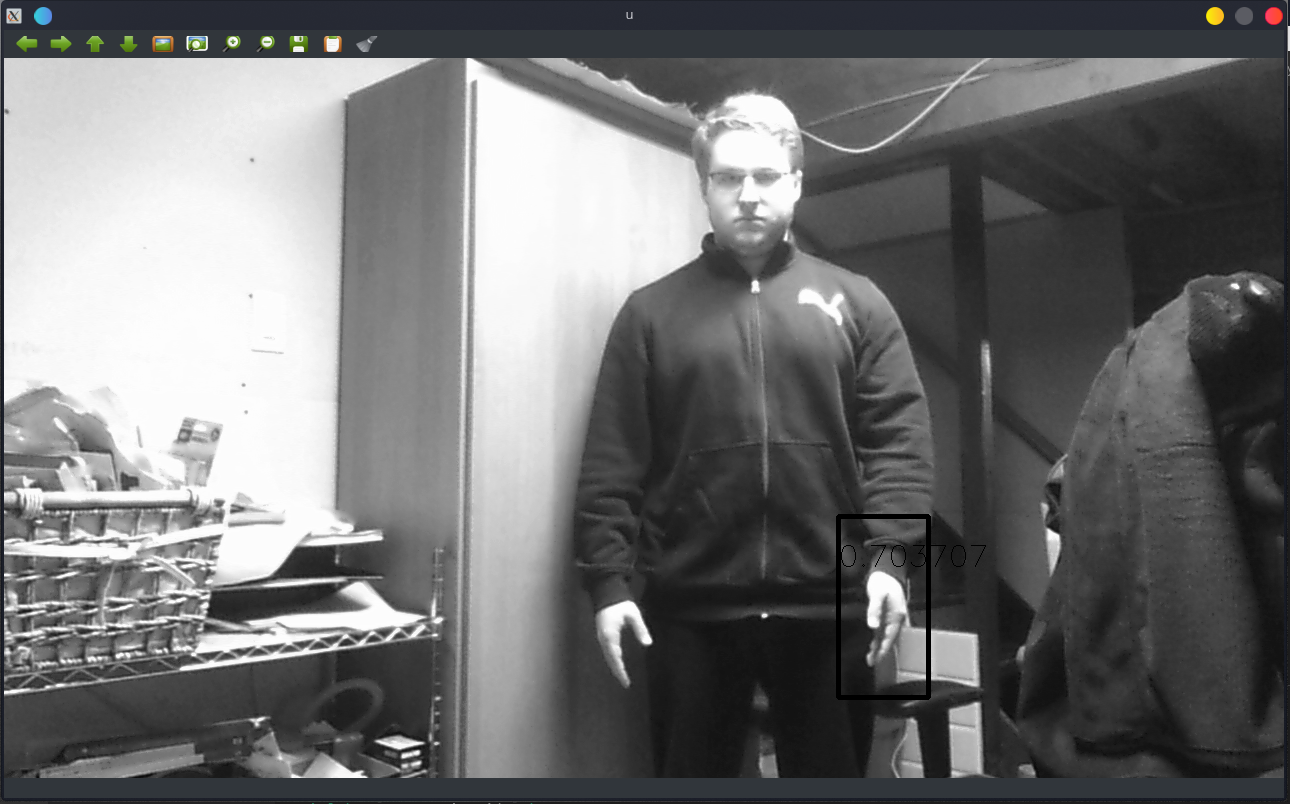
\includegraphics[width=\textwidth]{figures/PT_webcam_hand.png}
%     \caption{Hand Detection Error}
% \end{figure}

Later, testing started to use video files to be more in line with how we wanted to achieve this project. The video used was of a motorcyclist who had a camera attached to their helmet and was riding around while driving by careless pedestrians. When viewing the results of the video file, the accuracy of the HOG descriptor was much more in line with what we had hoped. Most if not all of the pedestrians were identified when within an acceptable range. Whenever the pedestrian tracking component produced a false negative, the cases that generated such errors were those where either a pedestrian was too far from or too close to the camera, and whenever the pedestrian was partially occluded. Both of these conditions are not out of the ordinary since being to close to the camera results in some occlusion since the pedestrian will be partially in frame. When to far away, the gradients in the HOG descriptor become harder to determine if they are human-shaped objects which is normal in nature. Partial occlusion of a pedestrian in the frame is also normal as parts of the gradient data is lost due to occlusion.

\subsection{Road Sign Tracking}